%--------------------------------------------------------------------
%--------------------------------------------------------------------
% Formato para los talleres del curso de Métodos Computacionales
% Universidad de los Andes
%--------------------------------------------------------------------
%--------------------------------------------------------------------

\documentclass[11pt,letterpaper]{exam}
\usepackage[utf8]{inputenc}
\usepackage[spanish]{babel}
\usepackage{graphicx}
\usepackage{tabularx}
\usepackage[absolute]{textpos} % Para poner una imagen en posiciones arbitrarias
\usepackage{multirow}
\usepackage{float}
\usepackage{hyperref}
%\decimalpoint

\begin{document}
\begin{center}
{\Large Métodos Computacionales} \\
\textsc{Tarea 2}\\
Maria Camila Garcia 201515657\\
11-05-2019\\
\end{center}

En la siguiente figura se presenta la grafica de los datos signal.dat y signalSuma.dat.

\noindent
\section{Ejercicio 1: Fourier}
\begin{center}
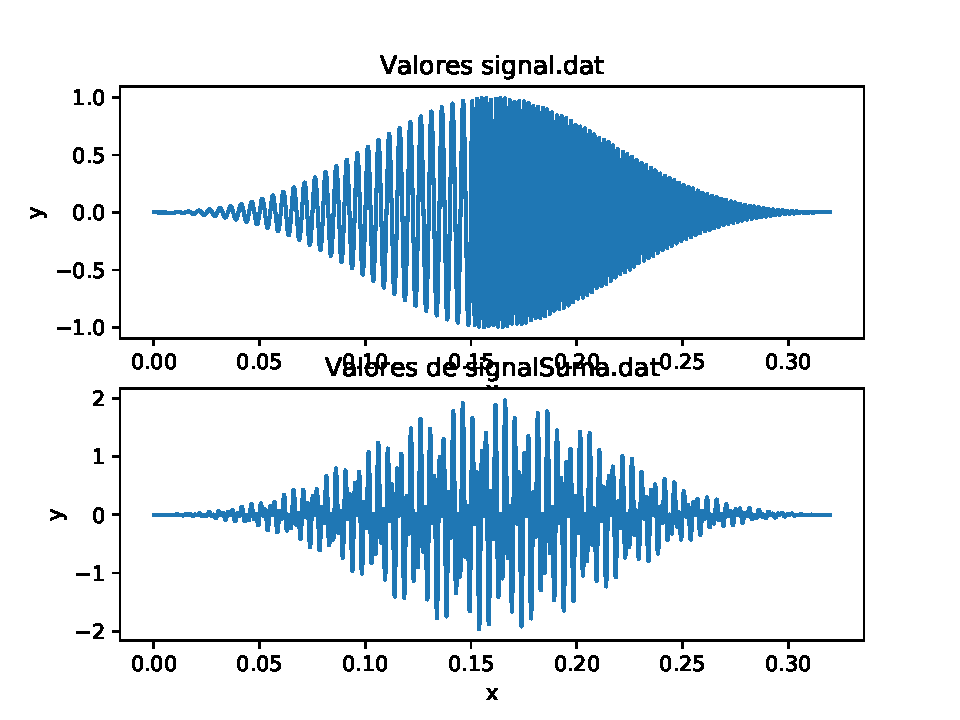
\includegraphics[width=10cm]{GarciaCamila_SubplotsGraficas.pdf}
\end{center}

A continuacion se tienen la grafica de de las transformadas de fourier para ambas señales. 

\begin{center}
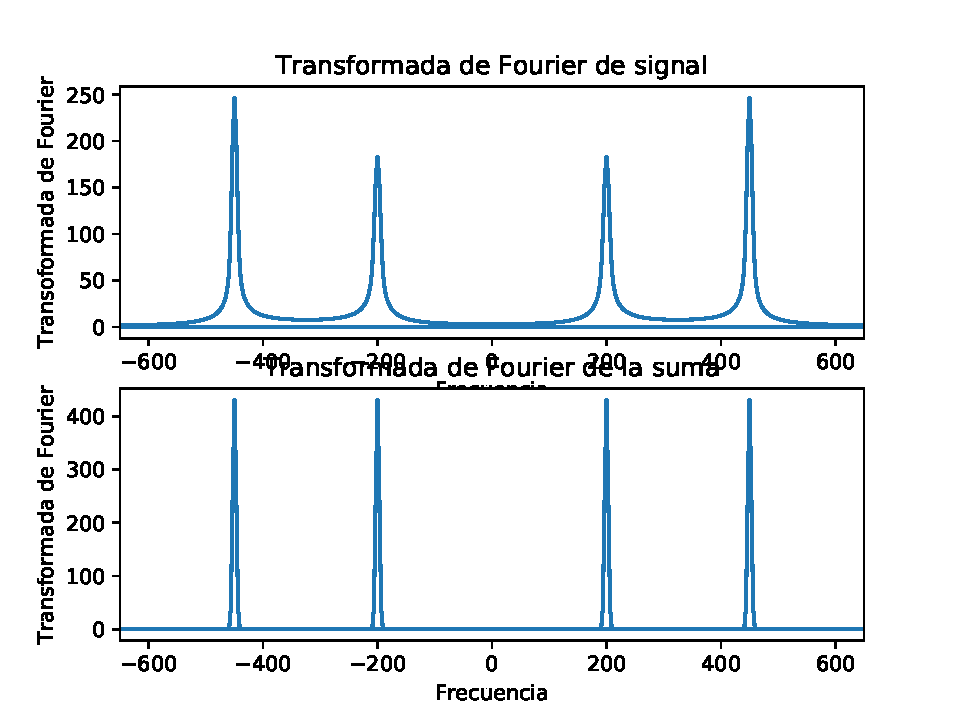
\includegraphics[width=10cm]{GarciaCamila_Transformadas.pdf}
\end{center}

La anterior transformada de Fourier cumplio con el objetivo de simplificar las amplitudes de la grafica original.

Posteriormente, se muestra el espectrograma de los datos signal.dat y signalSuma.dat.

\begin{center}
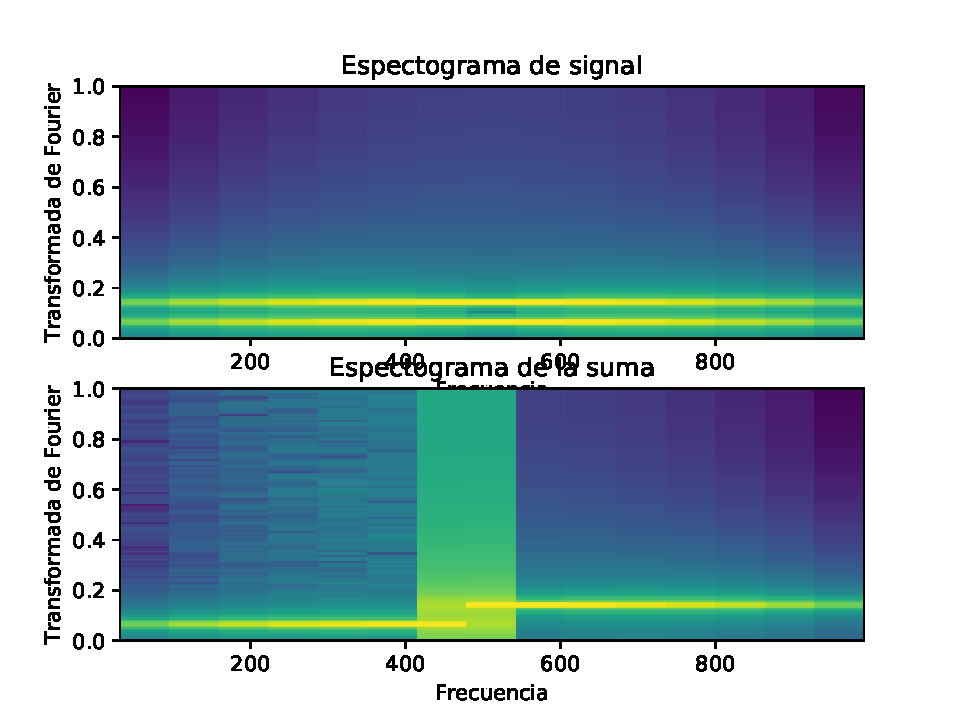
\includegraphics[width=10cm]{GarciaCamila_Espectrogramas.pdf}
\end{center}

En la grafica de la señal en funcion del tiempo de temblor.txt se tiene:

\begin{center}
\includegraphics[width=10cm]{GarciaCamila_Temblor.pdf}
\end{center}

\begin{center}
\includegraphics[width=10cm]{GarciaCamilaTransformadaTemblor.pdf}
\end{center}

Al igual que las graficas de la funcion anterior, la transformada de Fourier elimino datos que no son del todo utiles y simplifico la lectura de los datos.

\begin{center}
\includegraphics[width=10cm]{GarciaCamila_EspectrogramaTemblor.pdf}
\end{center}

Respecto a ambos espectrogramas, pordemos decir que para el caso del temblor, este busca medir el movimiento de la estructura ante la vibracion del suelo que soporta. En general, representa la energia del contenido de la señal, por lo que hace un trabajo muy similar al de la transformada de Fourier. Los valores mas oscuros representan un valor negativo, mientras que los valores mas claros representan valores positivos.


\noindent
\section{Ejercicio 2: Ecuaciones diferenciales ordinarias: un edificio en un sismo}

La siguiente grafica es de la amplitud maxima en funcion de omega. 
\begin{center}
\includegraphics[width=10cm]{GarciaCamila_Amplitudui(t)maxVsW.pdf}
\end{center}

Como se puede ver en la grafica hay 3 picos importates de w, los cuales fueron seleccionados para hacer las demas graficas, siendo estos 0.8, 1.8 y 2.6. El primer pico lo genera u3 maximo, el segundo u1 maximo y el tercero u2 maximo.

\begin{center}
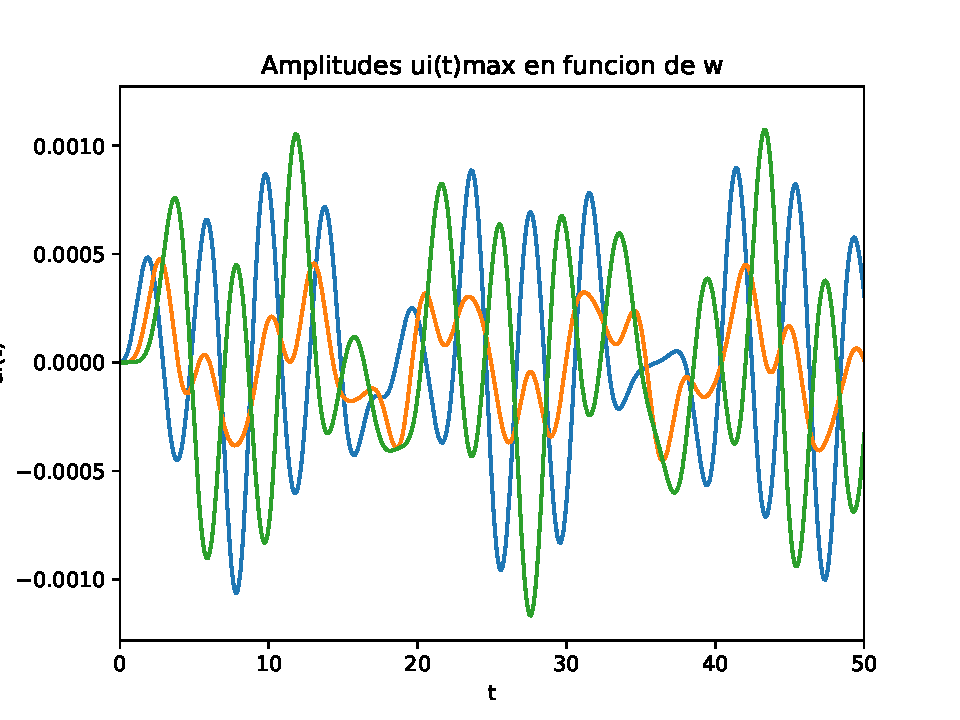
\includegraphics[width=10cm]{PrimeraGraficaUi(t).pdf}
\end{center}

Para esta primera grafica, se utilizo omega = $\sqrt{\frac{k}{m}}$, la cual es la ecuacion de una frecuencia angular de un resorte ideal que oscila, por lo que el movimiento es simple y armonico. En general no hay un patron respecto a la amplitud de este dato, en general el de menor amplitud es u2, mientras que u1 y u3 tienen una amplitud similar mas grande.

\begin{center}
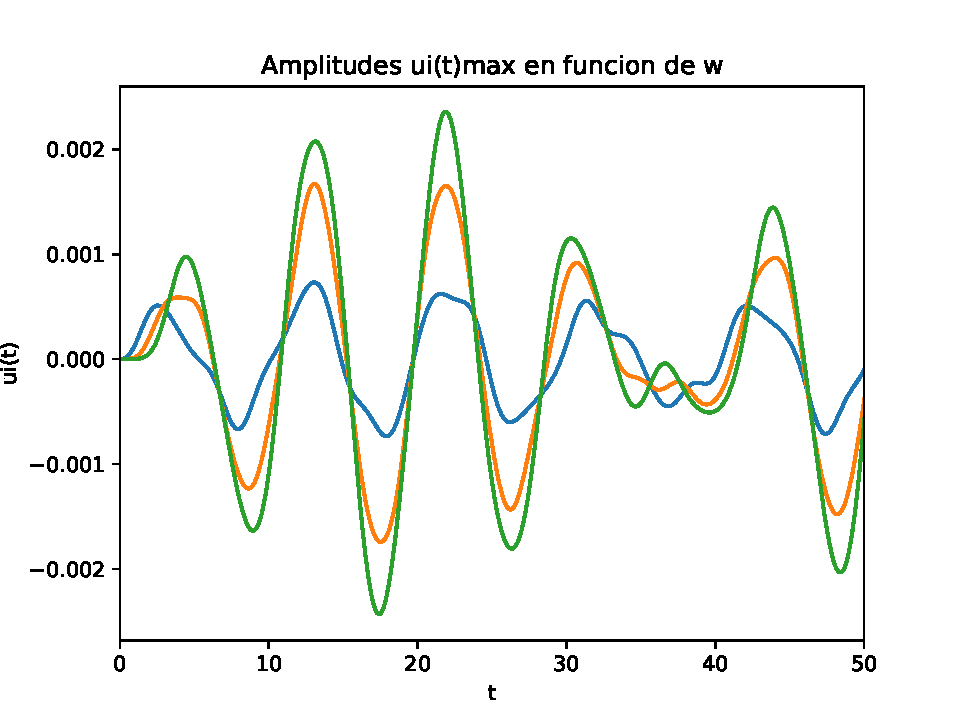
\includegraphics[width=10cm]{SegundaGraficaUi(t).pdf}
\end{center}

Para la anterior grafica, se tuvo en cuenta el primer pico de la grafica de amplitudes maximas, es decir 0.8. Se puede ver que u2 y u3 tienen valores muy similares, mientras que u1 presenta menor amplitud y son menos homogeneas entre si. 

\begin{center}
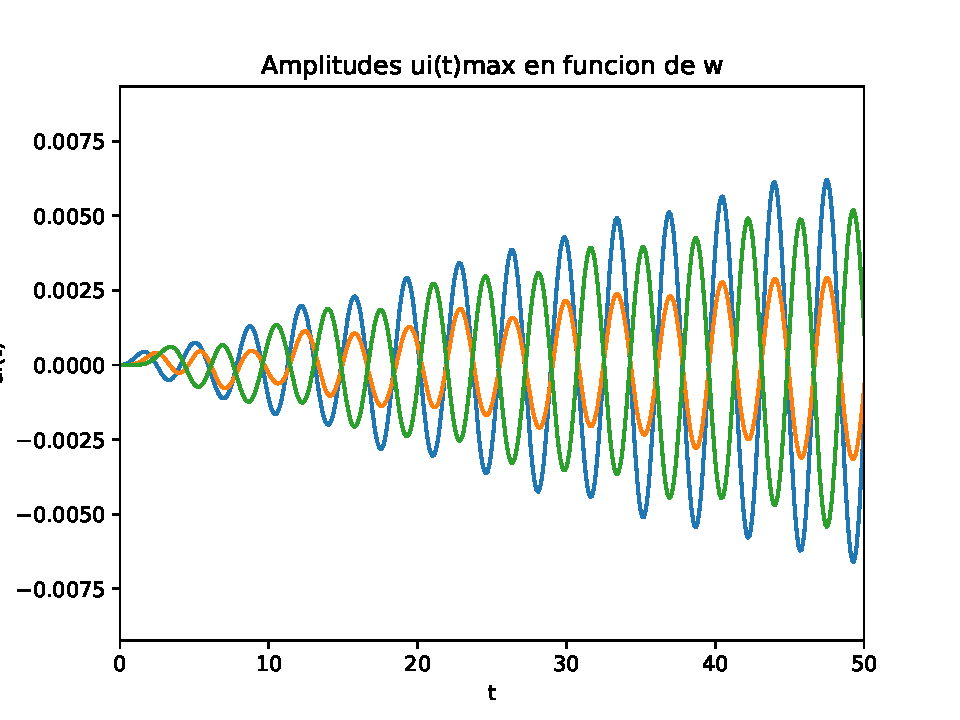
\includegraphics[width=10cm]{TerceraGraficaUi(t).pdf}
\end{center}

Para esta grafica, se utilizo como omega el valor de 1.8, para todos los valores de u hay un aumento de amplitud constante. 

\begin{center}
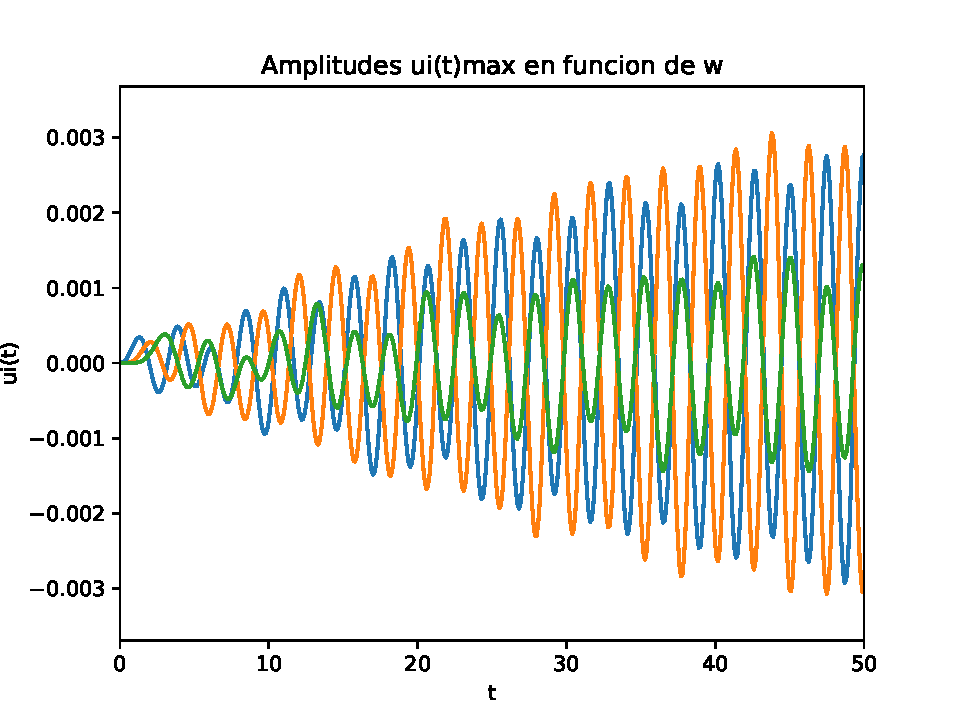
\includegraphics[width=10cm]{CuartaGraficaUi(t).pdf}
\end{center}

Para la grafica final, se utilizo el valor de omega de 2.6, este valor genero que la grafica tenga un aspecto muy parecido al de la anterior, hay un aumento constante pero el periodo se cumple en menor tiempo del de la anterior, que toma mas tiempo, u2 y u1 tienen mas amplitud que u3. 

\section{Bono: animacion, archivo Bono.py}
Se creo una animacion de como seria el movimiento del edficio con los datos del temblor. Teniendo en cuenta que el edificio es de tres pisos, se crearon dicho numero de linspace para poder crearlos, posteriormente se creo el movimiento de cada una de las paredes en el caso del sismo. 

Respecto a la animacion, no encontre un comando que me sirviera del todo par guardarla, cuando lo intentaba se quedaba estatica o simplemente no se guardaba.

Pero como se puede ver en la imagen, el edificio oscila de una lado a otro y cada vez que se aumenta la altura, aumenta tambien la oscilacion, es por esta razon que cuando hay un sismo, las personas en los pisos mas altos lo sientan con mayor intensidad.

\end{document}
